\chapter{Proposta Experimental}
\label{chap:proposta_experimental}

Este capítulo traz informações relacionadas com as ferramentas utilizadas no experimento, como linguagem, biblioteca, entre outros. Informações sobre o conjunto de dados \gls{ACDC}, utilizado como linha de base, e o conjunto de dados \gls{InCor}, que será utilizado em experimentos futuros. Por fim, são apresentados resultados experimentais com o conjunto de dados \gls{ACDC}. 

%--------------------------------------------------------
\section{Materiais} 
\label{sec:cap5_materiais}

Esta seção visa trazer informações sobre tanto o \textit{hardware} quanto o \textit{software}, como também as principais bibliotecas utilizadas e suas versões nos experimentos para fins de reprodução. A Tabela \ref{tab:hardware_software} estrutura estas informações.

\begin{table}[hbtp]
    \centering
    \renewcommand{\arraystretch}{1} % default é 1 
    % \begin{tabular}{|>{\centering\arraybackslash}p{2cm}|p{12cm}|}
    \begin{tabular}{|c|c|}
    \hline 
       \textbf{Item} & \textbf{Descrição}\\
    \hline 
       Computador & \textit{Macbook M1 Pro}  \\
    \hline 
       Memória & 16gb  \\
    \hline 
       Versão \textit{Python} & 3.11.0  \\
    \hline 
       Versão \textit{pyradiomics} & 3.0.1 \\
    \hline 
       Versão \textit{torch} & 2.2.1 \\
    \hline 
       Versão \textit{torchvision} & 0.17.1 \\
    \hline 
       Versão \textit{numpy} & 1.26.4 \\
    \hline 
       Versão \textit{scikit-learn} & 1.4.1.post1 \\
    \hline 
    \end{tabular} 
    \caption{Fonte: Autor}
    \label{tab:hardware_software}
\end{table}

%--------------------------------------------------------
\section{Conjunto de Dados} 
\label{subsec:cap5_dataset}

Este trabalho visa realizar os experimentos em duas bases distintas com imagens de \gls{RMC}, informações a cerca do paciente e rótulos que indicam presença ou não de cardiomiopatia. O primeiro conjunto de dados é o \gls{ACDC} e será utilizado como linha de base para avaliação da metodologia. O conjunto de dados para treino do \gls{ACDC} possui $30$ casos de \gls{CMH}, $30$ casos de \gls{CMD} e $90$ casos normais. Da base \gls{ACDC} se pretende utilizar apenas as fatias da fase diastólica. O segundo conjunto de dados é o \gls{InCor}, possuindo imagens na fase diastólica contendo as mesmas três classes de interesse previamente mencionadas. 

%--------------------------------------------------------
\subsection{Experimentos ACDC}
\label{subsec:cap5_experimentos_acdc}

A partir da arquitetura proposta foi realizada uma prova de conceito utilizando o conjunto de treino do \gls{ACDC} como linha de base, composto por $100$ exames de pacientes, coletando apenas as fatias das imagens da fase diastólica e a máscara referente disponibilizada. Características de primeira ordem e \gls{GLCM} são extraídas compondo ao todo $\RadiomicFeatures$ valores que compõem as características radiômicas. Para extração das características profundas, é utilizada uma rede \textit{ResNet50} congelada e sua última camada densa é removida, visto que originalmente esta é responsável pela predição das 1000 classes oriundas do conjunto de dados do \textit{ImageNet}. A rede, após adaptada, passa a produzir $\DeepFeatures$ características.

O \textit{F-Test} é utilizado como seletor de características, aplicado tanto nas características radiômicas quanto nas profundas, selecionando um total de $\SelectedFeatures$ características em cada abordagem: radiômicas e profundas. Essas características são concatenadas, enviadas ao módulo de autoatenção e os resultados armazenados.

Neste experimento foi treinado o modelo utilizando, como função objetivo a entropia cruzada binária, taxa de aprendizado de $\LR$, otimizador \textit{Adam}, tamanho de lote $\Batch$ e o treinamento se deu em aproximadamente $\Epochs$ épocas, onde verificou que o erro se torna estável. Também foi empregada a estratégia de aleatorizar as entradas do modelo e descartar o último lote caso ele não alcance o tamanho especificado para o mesmo. Com a saída do modelo é aplicada a função sigmoide, Equação. \ref{eq:sigmoide}, função esta que limita os valores de sua entrada entre 0 e 1. Para fins de classificação, valores maiores que $0,5$ são considerados com \gls{CMH} e menor ou iguais considerados normal.

\begin{equation}
\textit{sigmoide}(x) = \frac{1}{1 + e^x}
\label{eq:sigmoide}
\end{equation}

%--------------------------------------------------------
\section{Cronograma}
\label{sec:cronograma}

O cronograma proposto das atividades segue na Figura \ref{fig:fig014}. Os itens em azul são atividades concluídas como: disciplinas, revisão bibliográfica, refinamento do tema, testes iniciais, etc. Itens em rosa são atividades em andamento como: implementação de modelos de comparação e escrita da dissertação. Atividades em amarelo são atividades planejadas como: análise de resultados, escrita da dissertação e escrita de artigos.

\begin{figure}[htbp]
    \centering
    \caption{Cronograma planejado}
    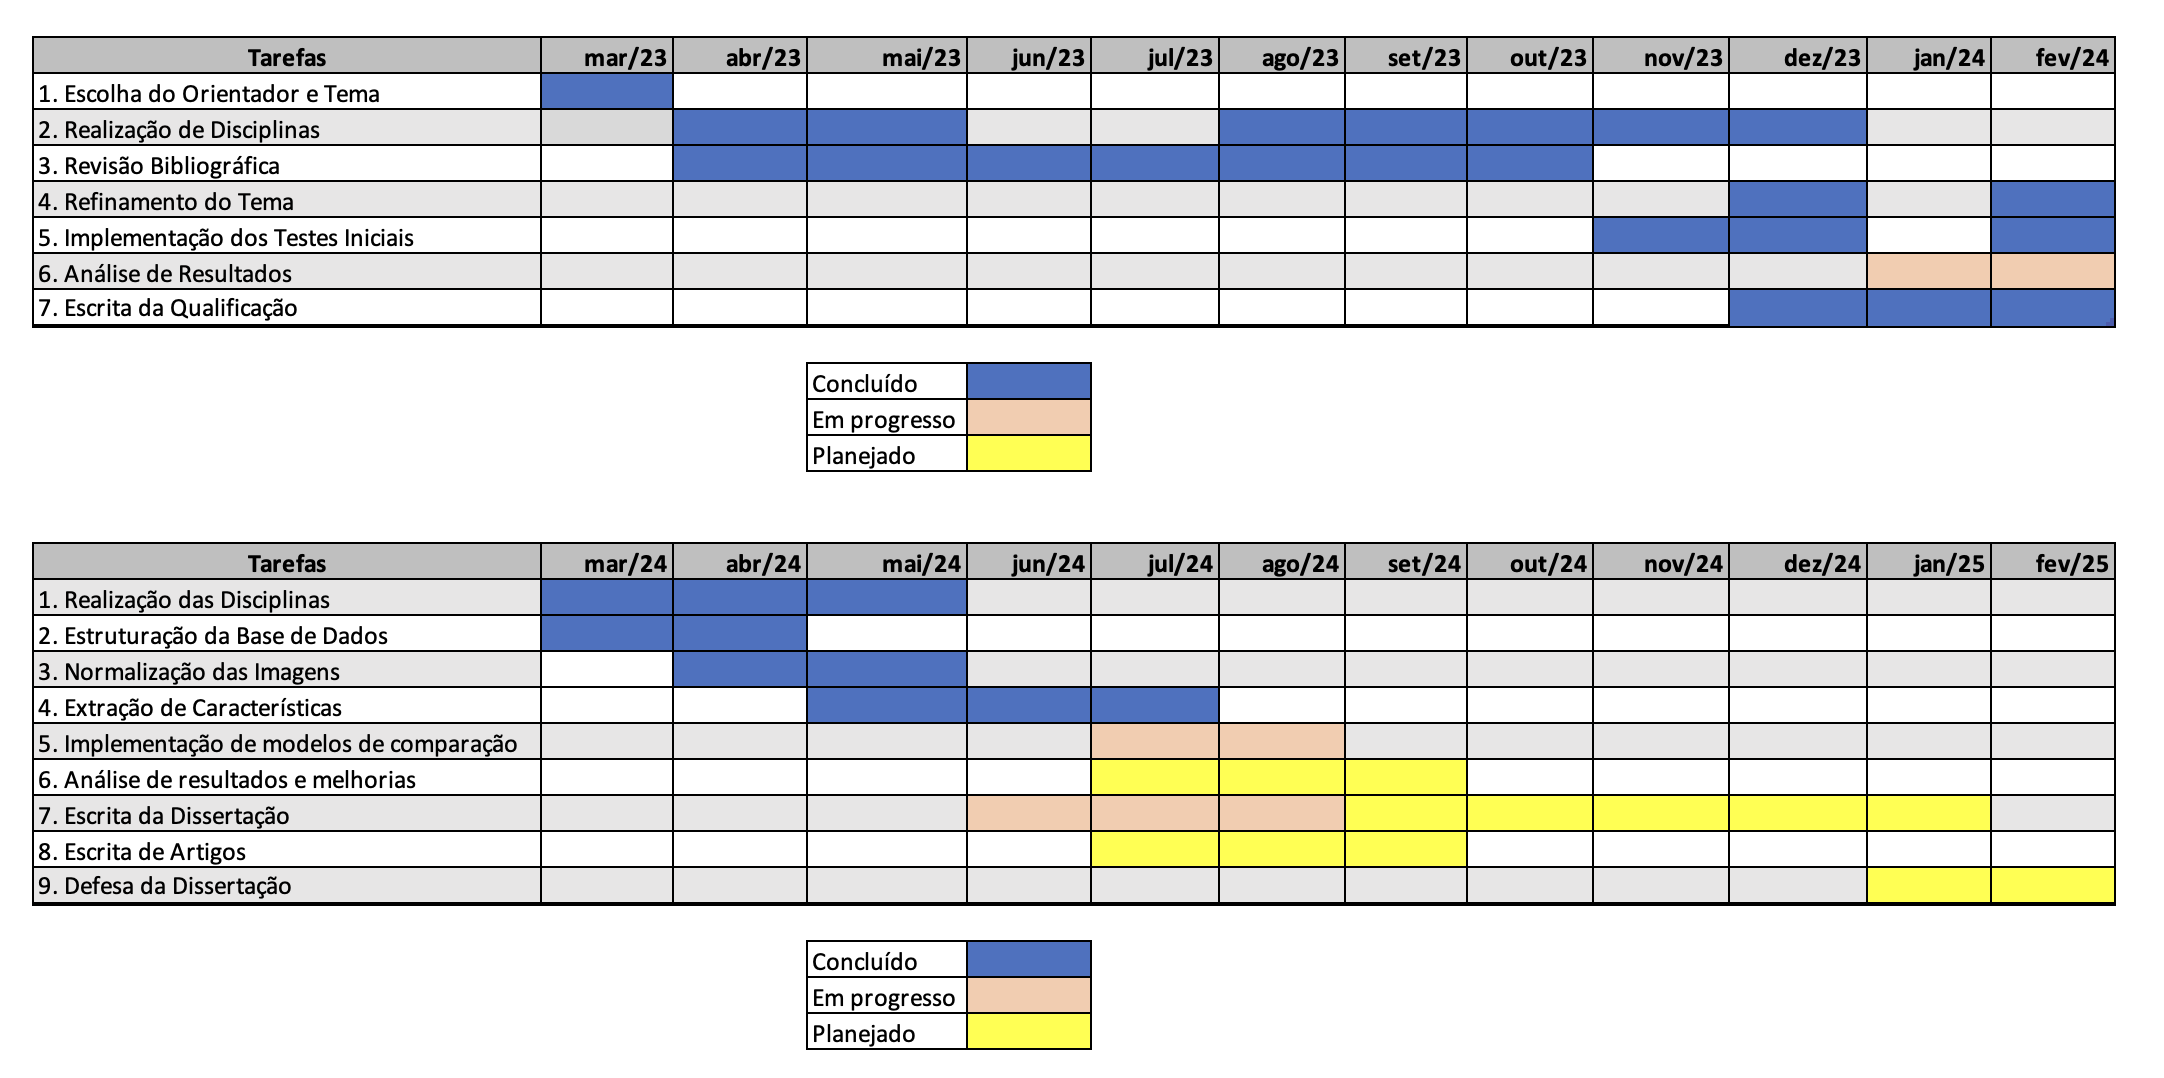
\includegraphics[width=1\textwidth]{figures/fig014.png}
    \caption*{Fonte: Autor}
    \label{fig:fig014}
\end{figure}
